% WaveOrder label-free screening whitepaper: 2-page print layout.
% The docs-site version of this tutorial is labelfree-screening.md; this
% file re-lays the same content and figures for a compact PDF.
% Uses only base texlive packages (no tcolorbox/titlesec on the build host).
\documentclass[9pt]{extarticle}
\usepackage[letterpaper,margin=1.25cm,bottom=1.8cm]{geometry}
\usepackage[T1]{fontenc}
\usepackage{textcomp}
\usepackage{helvet}
\renewcommand{\familydefault}{\sfdefault}
\usepackage{graphicx}
\usepackage{xcolor}
\usepackage{fancyvrb}
\usepackage{booktabs}
\usepackage[labelfont=bf,labelsep=period,font=small,skip=3pt]{caption}
\usepackage{enumitem}
\setlist{nosep,leftmargin=1.2em}
\usepackage{fancyhdr}
\usepackage[colorlinks=true,linkcolor=black,urlcolor=blue!60!black]{hyperref}
\setlength{\parindent}{0pt}
\setlength{\parskip}{4pt}
\pagestyle{fancy}
\fancyhf{}
\renewcommand{\headrulewidth}{0pt}
\fancyfoot[L]{\raisebox{-3pt}{
\includegraphics[height=13pt]{brand/biohub-logo-black.png}}}
\fancyfoot[R]{\small Computational Imaging Team \textbar{} \texttt{\{talon.chandler,shalin.mehta\}@biohub.org} \textbar{} 2026-11-13}

\definecolor{boxgray}{gray}{0.96}
\definecolor{boxframe}{gray}{0.75}
\newcommand{\mysection}[1]{\vspace{5pt}{\Large\bfseries #1}\par\vspace{2pt}}
\setlength{\fboxsep}{6pt}
\setlength{\fboxrule}{0.4pt}

% Verbatim blocks saved up front so they can live inside boxes.
\begin{SaveVerbatim}{cfgyml}
input_channel_names: [BF]
reconstruction_dimension: 2
phase:
  transfer_function:
    yx_pixel_size: 0.325  # 6.5 um / 20x
    z_pixel_size: 2.0
    wavelength_illumination: 0.450
    index_of_refraction_media: 1.0
    numerical_aperture_detection: 0.55
    numerical_aperture_illumination: 0.4
    invert_phase_contrast: false
    z_focus_offset: auto
  apply_inverse:
    regularization_strength: 0.001
\end{SaveVerbatim}

\begin{SaveVerbatim}{tiltcfg}
    z_focus_offset: auto
    tilt_angle_zenith:  {init: 0.13, lr: 0.05}
    tilt_angle_azimuth: {init: 0.0,  lr: 0.05}
optimization: {max_iterations: 50, method: adam}
\end{SaveVerbatim}

\begin{document}

{\huge\bfseries WaveOrder for label-free high-throughput screening}

\vspace{5pt}
This guide demonstrates WaveOrder for label-free high-throughput
screening using optical pooled screening (OPS) data from the
\href{https://www.biorxiv.org/content/10.64898/2026.06.01.728087v1}{Biohub's multimodal
perturbation atlas} [1], where phase from defocus enabled label-free tracking and
phenotyping of CRISPR-perturbed A549 cells. Brightfield
defocus stacks from a standard motorized widefield microscope, together with a
\href{https://github.com/biohub/waveorder}{WaveOrder} config [2], yield
quantitative phase at screening scale (Figure~1).

After reading this guide and acquiring data, use the
\href{https://github.com/biohub/waveorder/blob/main/docs/guide/first-reconstruction.md}{first-reconstruction
guide} and connect your agent to the
\href{https://biohub.ai/mcp}{Biohub MCP} to run the
\texttt{waveorder-tutorial} skill. Methods are described in the
\href{https://arxiv.org/abs/2412.09775}{WaveOrder preprint} [3].

\begin{figure}[h!]
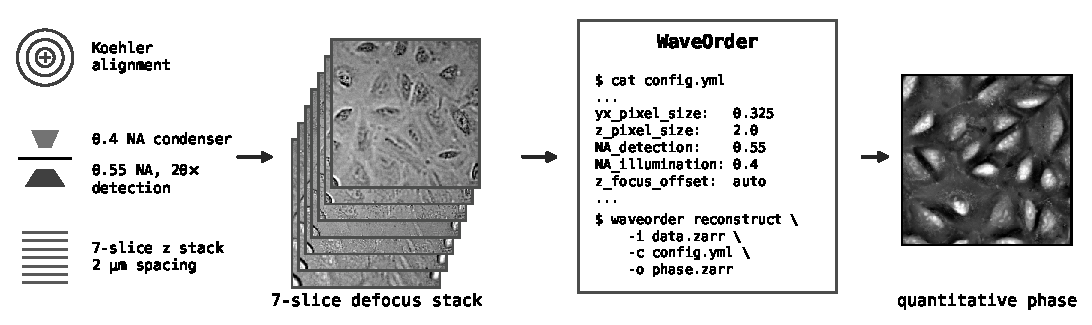
\includegraphics[width=\linewidth]{figures/fig_overview.pdf}
\caption{Key acquisition settings (left) produce a defocus stack with
defocus-dependent contrast that WaveOrder converts into quantitative phase.}
\end{figure}

\mysection{Acquisition}

The three settings that matter most are:
\begin{itemize}
\item \textbf{Koehler illumination.} Align the condenser before every
  session. Misalignment is the most common source of artifacts. Ron Vale's
  five-minute
  \href{https://www.ibiology.org/talks/set-up-koehler-illumination/}{iBiology
  tutorial} [4] is a good refresher.
\item \textbf{Condenser NA $\approx$ 2/3 of detection NA.} We used a 0.4 NA condenser and
  a 0.55 NA objective. A larger condenser aperture reduces contrast, while a
  smaller condenser aperture reduces contrast and resolution.
\item \textbf{Z spacing and range.} At 20$\times$, start at 2 \textmu m
  spacing and cover the full cell height with visibly blurred features on either end of the stack (here, 7 slices = 12 \textmu m).
  For different objectives, scale inversely with magnification: e.g.\, 4 \textmu m at 10$\times$, 1 \textmu m
  at 40$\times$.
\end{itemize}

\begin{table}[h!]
\small
\centering
\begin{tabular}{llp{2.7in}}
\toprule
Parameter & Perturbation atlas value & Notes \\
\midrule
Objective & 20$\times$, 0.55 NA, air & any objective works; match the config \\
Condenser & 0.4 NA & $\approx$2/3 of detection NA, Koehler aligned \\
Z stack & 7 slices, 2 \textmu m & confirm defocused features on top and bottom slices; use more slices for thicker samples \\
Camera & 6.5 \textmu m pixels & 6.5 \textmu m / 20$\times$ = 0.325 \textmu m at the sample \\
Wavelength & 450 nm & any wavelength is fine; ideally use a 10 nm notch filter \\
Exposure & a few ms & fill 1/2--2/3 of the dynamic range \\
\bottomrule
\end{tabular}
\caption{Acquisition parameters for the \href{https://www.biorxiv.org/content/10.64898/2026.06.01.728087v1}{Biohub's multimodal perturbation atlas dataset.}}
\end{table}

\mysection{Reconstruction}

\begin{minipage}[t]{0.55\linewidth}
Convert to OME-Zarr with
\href{https://github.com/czbiohub-sf/iohub}{iohub}
(\texttt{iohub convert -i <dataset> -o data.zarr}), record the acquisition
parameters in a config, reconstruct one position, and compare against the
raw data in napari:

\vspace{3pt}
\begin{Verbatim}[fontsize=\small]
waveorder reconstruct \
    -i data.zarr/A/1/029029 \
    -c config.yml -o phase.zarr
waveorder view data.zarr/A/1/029029 \
    phase.zarr/A/1/029029
\end{Verbatim}
\vspace{3pt}

Dense structures (nucleoli, nuclear envelopes, cell margins) should appear
brighter than background, as in Figure~1. \texttt{reconstruction\_dimension:~2} returns one
phase image per defocus stack, the best choice for samples that are thin compared to the depth of field of the microscope. If the sample appears to blur all at once as you defocus, use 2. If different regions of the sample blur at different defocus positions, consider trialling 3.
\end{minipage}\hfill
\begin{minipage}[t]{0.42\linewidth}
\vspace{0pt}
\fcolorbox{boxframe}{boxgray}{%
\begin{minipage}{\dimexpr\linewidth-2\fboxsep-2\fboxrule}
{\small\texttt{\$ cat config.yml}}\par\vspace{1pt}
{\small\UseVerbatim{cfgyml}}
\end{minipage}}
\end{minipage}

\vspace{8pt}
\noindent
\begin{minipage}[t]{0.555\linewidth}
\vspace{0pt}%
\fcolorbox{boxframe}{boxgray}{%
\begin{minipage}{\dimexpr\linewidth-2\fboxsep-2\fboxrule}
{\small\textbf{Failure mode 1 \textbar{} Flipped z axis}}\par\vspace{2pt}
\centering
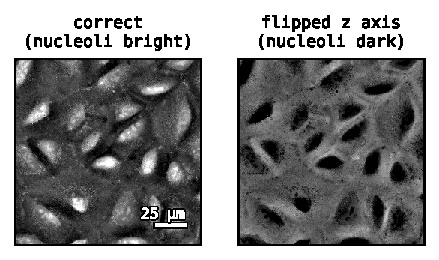
\includegraphics[width=0.97\linewidth]{figures/fig_flip.pdf}
\par\vspace{2pt}\raggedright\small
Stages disagree on the z sign convention---is the first slice above or below focus? If the convention is flipped, contrast
will be inverted and downstream comparison will be challenging. Dense organelles should be
bright. Fix: \texttt{invert\_phase\_contrast: true}. Check once per
microscope by reconstructing one stack both ways.
\end{minipage}}

\vspace{6pt}
\fcolorbox{boxframe}{boxgray}{%
\begin{minipage}{\dimexpr\linewidth-2\fboxsep-2\fboxrule}
{\small\textbf{Failure mode 3 \textbar{} Autofocus drift}}\par\vspace{2pt}
\centering
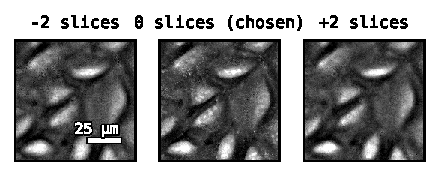
\includegraphics[width=0.97\linewidth]{figures/fig_focus.pdf}
\par\vspace{2pt}\raggedright\small
When the stack center (e.g. the 4th slice in a 7 slice stack) is not in focus, the reconstruction will be blurry.
Setting \texttt{z\_focus\_offset:~auto} runs
the search that can recover the defocus offset.
\end{minipage}}
\end{minipage}\hfill
\begin{minipage}[t]{0.425\linewidth}
\vspace{0pt}%
\fcolorbox{boxframe}{boxgray}{%
\begin{minipage}{\dimexpr\linewidth-2\fboxsep-2\fboxrule}
{\small\textbf{Failure mode 2 \textbar{} Incorrect regularization}}\par\vspace{2pt}
\centering
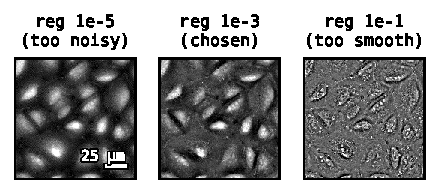
\includegraphics[width=0.97\linewidth]{figures/fig_reg.pdf}
\par\vspace{2pt}\raggedright\small
\texttt{regularization\_strength} balances noise and resolution and varies by
orders of magnitude across samples and exposures. Sweep decades on one
position and choose manually. Too small
amplifies blotchy low-frequency noise; too large leaves a washed-out image. The optimum is usually within a decade of
\texttt{1e-3}.
\end{minipage}}

\vspace{6pt}
\fcolorbox{boxframe}{boxgray}{%
\begin{minipage}{\dimexpr\linewidth-2\fboxsep-2\fboxrule}
{\small\textbf{Failure mode 4 \textbar{} Tilted illumination at the well edge}}\par\vspace{2pt}
\centering
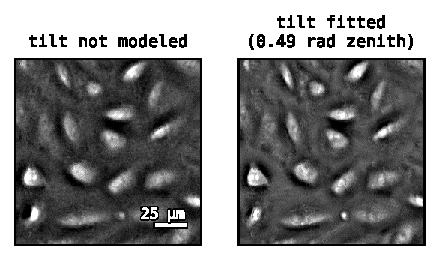
\includegraphics[width=0.97\linewidth]{figures/fig_tilt.pdf}
\par\vspace{2pt}\raggedright\small
Misaligned Koehler and imaging near a well-edge meniscus tilts the illumination, making cells look shadow-cast
with reduced contrast. Fit the tilt by gradient descent in the same config:
{\footnotesize\UseVerbatim{tiltcfg}}
\end{minipage}}
\end{minipage}

\mysection{Scaling up}

A single config file should generate good reconstructions across a screen. We suggest parallelizing
\texttt{waveorder reconstruct} over positions (one process or cluster job
per position) with \texttt{device:~cuda:0} to reconstruct on a GPU. We recommend
\texttt{z\_focus\_offset:~auto} to find the focus of each position.

We recommend manual supervision
to set up the optimized \texttt{tilt\_angle\_\{zenith,azimuth\}} parameters across entire wells. We find that initializing these tilt parameters at good initial tilts generates the stablest reconstructions, so we recommend inspecting
reconstructions at the well edges, then refining the initial values until you reach stable reconstructions that pass QC.

\mysection{References}

\sloppy
\begin{enumerate}
\item C.~Liu, A.~V.~Hillsley, M.~Sekhar, et al., ``A Multimodal Perturbation
  Atlas Defines the Phenotypic Resolution of Cellular Morphology,''
  \href{https://www.biorxiv.org/content/10.64898/2026.06.01.728087v1}{bioRxiv
  2026.06.01.728087}.
\item WaveOrder repository:
  \href{https://github.com/biohub/waveorder}{github.com/biohub/waveorder}.
\item T.~Chandler, I.~E.~Ivanov, G.~Sturm, et al.,
  ``WaveOrder: A differentiable wave-optical framework for scalable
  biological microscopy with diverse modalities,''
  \href{https://arxiv.org/abs/2412.09775}{arXiv:2412.09775}.
\item R.~Vale, ``Microscopy: Setting Up Koehler Illumination,''
  \href{https://www.ibiology.org/talks/set-up-koehler-illumination/}{iBiology
  Microscopy Series}.
\end{enumerate}

\end{document}
